\documentclass[11pt,a4paper]{article}
\usepackage[T1]{fontenc}
\usepackage{lmodern}
\usepackage[margin=25mm]{geometry}
\usepackage{amsmath,amssymb,amsthm,booktabs,graphicx,microtype}
\usepackage[colorlinks=true,linkcolor=blue!50!black,citecolor=blue!50!black,urlcolor=blue!50!black]{hyperref}
\usepackage{xcolor}
\usepackage{enumitem}
\setlist{nosep}
\setlength{\emergencystretch}{2em}
\clubpenalty=10000
\widowpenalty=10000
\displaywidowpenalty=10000
\renewcommand{\topfraction}{.85}
\renewcommand{\textfraction}{.12}
\renewcommand{\floatpagefraction}{.95}
\setcounter{totalnumber}{1}
\newtheorem{theorem}{Theorem}
\newtheorem{proposition}[theorem]{Proposition}
\newtheorem{lemma}[theorem]{Lemma}
\newcommand{\E}{\mathbb E}
\newcommand{\Var}{\operatorname{Var}}
\newcommand{\Cov}{\operatorname{Cov}}
\newcommand{\Pois}{\operatorname{Pois}}
\title{Failure-Conditioned Count Measurements\\at the Peeling Threshold}
\author{Min Wu}
\date{Working paper, version 0.1\\October 1, 2026}
\begin{document}
\maketitle
\begin{abstract}
Count measurements in invertible lookup sketches may be consulted only after peeling fails. This selection can change their distribution even when the unconditional mean and variance do not depend on the sign composition. We study independent uniform $k$-subset mappings in the critical window of ideal degree-one peeling, for fixed $k\ge3$ and deterministic signs independent of the mapping. The central result is a joint Gaussian limit for normalized count energy and a precritical score that determines failure asymptotically. The failure-conditioned measurement then follows a Gaussian-selection law with explicit correlation $\eta_k\rho^2$, where $\rho$ is the limiting sign imbalance. The correlation changes sign between $k=4$ and $k=5$, reversing the direction of conditional mean and limiting quantile shifts. A separate balanced-sign result gives invariance under symmetric mapping events whose probabilities stay bounded away from zero. Numerical experiments examine lower-tail calibration and expose limitations of finite-size approximations. This working paper presents the main results and their proof arguments; it does not provide a uniform finite-size risk guarantee.
\end{abstract}

\section{Introduction}
An invertible lookup sketch recovers its input by repeatedly removing an element identified through a degree-one cell. If peeling stops before all elements have been removed, the count array can still contain useful information about the input size. A statistical difficulty arises when the measurement is consulted only after failure: the decision to use the measurement and the measurement itself depend on the same random mapping. An unconditional reference distribution need not describe the measurements actually used by this decision rule.

We study the count energy measured \emph{before peeling}, conditioned on the eventual failure of ideal degree-one peeling. The observable includes the entire initial mapping, and the target $d$ is the initial number of elements. It is not a measurement of the number of edges in the residual core. Positive and negative signs determine the contributions of individual elements to the count array. Failure depends on the unsigned mapping, whereas energy depends on both the mapping and the signs.

The exact conditional mean has a simple projection onto sign imbalance, but a mean identity does not determine a conditional distribution. Near the peeling threshold, the number of elements and the number of cells grow together while failure retains a nontrivial limiting probability. Selection can therefore retain a persistent component of the standardized measurement fluctuation.

Finite-size scaling for random hypergraph cores and iterative decoding already describes the leading critical failure probability~\cite{dm,amru}. Covariance evolution also has established analytic methods~\cite{nks}. The additional question here is how an external statistic of the initial mapping fluctuates \emph{jointly} with the score controlling failure. Neither the marginal failure probability nor a covariance calculation alone answers this question.

Our main result connects count energy to actual peeling failure in the Plain mapping model. Its explicit correlation identifies two effects: sign imbalance attenuates selection by a factor $\rho^2$, and changing $k$ from four to five reverses its direction. A graph-conditional sign limit also yields a balanced-selection invariance result independently of the peeling dynamics. We use these results to interpret lower-tail calibration, distinguishing limiting predictions from empirical finite-size corrections.

The distributional formula is a classical Gaussian-selection expression. The contribution lies in establishing the measurement--failure connection for this mapping model and identifying its parameter. The accompanying \href{https://github.com/whitewum/peeling-lens}{Peeling Lens} laboratory provides an interactive view of the trajectories and fluctuation decomposition.

\section{Model and exact identities}
\subsection{Plain mappings and ideal peeling}
Let $M$ be the number of cells and $d$ the number of elements. Element $i$ independently chooses a uniformly distributed $k$-subset $S_i\subseteq[M]$. Repeated endpoints within an edge are forbidden, but different elements may choose identical subsets. We call this the Plain model.

Ideal degree-one peeling repeatedly removes an edge incident to a degree-one vertex. Let $F_M$ be the event that a nonempty residual hypergraph remains. This event is equivalent to a nonempty residual 2-core and does not depend on the order of leaf removal. It is independent of signs and invariant under permutations of element labels. Nonideal purity or checksum decisions are outside the model.

For deterministic signs $s_i\in\{-1,+1\}$ independent of the mapping, define
\begin{equation}
\rho_M=\frac1d\sum_{i=1}^d s_i,\qquad C_v=\sum_{i:v\in S_i}s_i.
\end{equation}
The initial count energy and standardized measurement are
\begin{align}
T_M&=\sum_{v=1}^M\left(C_v-\frac{kd\rho_M}{M}\right)^2,\label{eq:energy}\\
\widehat d_M&=\frac{T_M}{k(1-k/M)},\qquad X_M=\frac{\widehat d_M-d}{s_M},
\qquad s_M^2=\frac{2d(d-1)}{M-1}.\label{eq:measurement}
\end{align}
The centering term is available from $\sum_v C_v=kd\rho_M$. The notation $s_M$ denotes the standard deviation, whereas $s_i$ denotes an element sign.

\subsection{Sign-independent first two moments}
For $M>k$ and $d\ge2$, the Plain model gives $\E X_M=0$ and $\Var X_M=1$ for every fixed sign vector. To see this, let $H_{ij}=|S_i\cap S_j|$. Then
\begin{equation}
T_M=kd(1-k/M)+2\sum_{i<j}s_is_j(H_{ij}-k^2/M).
\end{equation}
The hypergeometric distribution gives
\begin{equation}
\E H_{ij}=k^2/M,\qquad
\Var H_{ij}=\frac{k^2(M-k)^2}{M^2(M-1)}.
\end{equation}
Distinct unordered pairs are uncorrelated, including pairs sharing one element: conditional on that element's mapping, both conditional means remain $k^2/M$. Summing the variances proves the normalization in~\eqref{eq:measurement}.

For any unsigned mapping event $A$ of positive probability that is invariant under element-label permutations, define
\begin{equation}
c_A=\frac{\E[H_{12}\mid A]-k^2/M}{k(1-k/M)}.
\end{equation}
Exchangeability and $2\sum_{i<j}s_is_j=d^2\rho_M^2-d$ imply the exact identity
\begin{equation}
\frac{\E[\widehat d_M\mid A]}d-1=c_A(d\rho_M^2-1).\label{eq:projection}
\end{equation}
This controls the conditional mean but not the full conditional law.

\section{The critical-window limit}
\subsection{Constants and main result}
Fix an integer $k\ge3$. Let $x_c$ be the unique positive root of
$e^{x_c}-1=(k-1)x_c$, and set
\begin{equation}
q_c=1-e^{-x_c},\quad a_c=q_c^{k-1},\quad
\mu_c=x_c/a_c,\quad\alpha_c=\mu_c/k.
\end{equation}
We consider deterministic sequences satisfying
\begin{equation}
\frac dM=\alpha_c+\frac r{\sqrt M}+o(M^{-1/2}),\qquad
r\in\mathbb R,\qquad\rho_M\longrightarrow\rho\in[-1,1].\label{eq:window}
\end{equation}
The window parameter $r$ is fixed. A small positive limiting failure probability is allowed; a probability tending to zero is not covered.

\begin{theorem}[Joint measurement--failure limit]\label{thm:main}
Under these assumptions, there is an unsigned, element-label-invariant precritical score $R_M$ such that
\begin{align}
\left(X_M,\frac{R_M-\beta_k r}{\sigma_k}\right)
&\Rightarrow N\!\left(0,\begin{pmatrix}1&\eta_k\rho^2\\\eta_k\rho^2&1\end{pmatrix}\right),\label{eq:joint}\\
\Pr\bigl(F_M\triangle\{R_M\le0\}\bigr)&\longrightarrow0,\label{eq:transfer}
\end{align}
where
\begin{align}
\beta_k&=-ka_ce^{-x_c},\\
\sigma_k^2&=e^{-x_c}q_c\left(1-\frac{k a_c}{k-1}\right),\\
\eta_k&=\frac{e^{-x_c}a_c(x_c-2)}{\sqrt{2\sigma_k^2}}.\label{eq:eta}
\end{align}
With $z_r=-\beta_k r/\sigma_k$ and $c=\eta_k\rho^2$,
\begin{align}
\Pr(F_M)&\longrightarrow\Phi(z_r),\\
\sup_{x\in\mathbb R}\left|\Pr(X_M\le x\mid F_M)
-\frac{\Phi_2(x,z_r;c)}{\Phi(z_r)}\right|&\longrightarrow0.\label{eq:selection}
\end{align}
Here $\Phi$ and $\phi$ denote the standard normal CDF and density, and $\Phi_2(\cdot,\cdot;c)$ the standard bivariate normal CDF with correlation $c$.
\end{theorem}

Both~\eqref{eq:joint} and~\eqref{eq:transfer} are essential. The former identifies joint fluctuations; the latter connects the score to actual global failure. Together they give
$\Pr(X_M\le x,F_M)\to\Phi_2(x,z_r;c)$. Dividing by the positive limiting failure probability gives the conditional law. Continuity of the limiting CDF upgrades pointwise convergence to uniform convergence.

\subsection{Mean, quantiles, and sign reversal}
Write $A(z)=\phi(z)/\Phi(z)$. The exact second moment $\E X_M^2=1$ and the positive lower bound on $\Pr(F_M)$ imply uniform integrability of the conditional first moments. Hence
\begin{equation}
\E[X_M\mid F_M]\longrightarrow-\eta_k\rho^2A(z_r).\label{eq:mean}
\end{equation}
The limiting selection distribution has variance
$1-c^2A(z_r)[z_r+A(z_r)]$. This is a formula for the limiting law; bounded second moments alone do not imply convergence of finite-sample conditional variances.

\begin{table}[tbp]
\centering
\caption{Analytic constants, without simulation fitting. The dynamic variance $\tau_k^2$ is defined in~\eqref{eq:tau}.}
\begin{tabular}{rrrr}
\toprule
$k$ & $\sigma_k^2$ & $\tau_k^2$ & $\eta_k$\\
\midrule
3 & 0.047334402 & 0.031017361 & $-0.352023542$\\
4 & 0.022604525 & 0.016877142 & $-0.041540768$\\
5 & 0.014632421 & 0.011169746 & $+0.126662297$\\
6 & 0.010718241 & 0.008107775 & $+0.219499658$\\
\bottomrule
\end{tabular}
\end{table}

The sign of $\eta_k$ is the sign of $x_c-2$. The positive root increases with $k$, and comparison at $x=2$ gives $x_c<2$ for $k=3,4$ and $x_c>2$ for fixed $k\ge5$. For nonzero $\rho$, the limiting conditional mean is therefore positive for $k=3,4$ and negative for $k\ge5$. Applying~\eqref{eq:projection} in the one-sided case yields
\begin{equation}
M^{3/2}c_{F_M}\longrightarrow
-\frac{\sqrt2\eta_k}{\alpha_c}A(z_r).
\end{equation}
This is a critical-window statement, not a claim about every finite load.

Let $q_{\rm sel}(u;z,c)$ denote the level-$u$ quantile of $\Phi_2(x,z;c)/\Phi(z)$. Its density is
\begin{equation}
f_{\rm sel}(x;z,c)=\frac{\phi(x)}{\Phi(z)}
\Phi\!\left(\frac{z-cx}{\sqrt{1-c^2}}\right),
\end{equation}
which is strictly positive. Consequently, conditional quantiles converge at every fixed $u\in(0,1)$. The identity
$\partial_c\Phi_2(x,z;c)=\phi_2(x,z;c)>0$
shows that positive $c$ shifts every limiting quantile below the standard normal counterpart, and negative $c$ shifts it above. For one-sided signs and $k\ge5$, an unconditional normal lower-tail threshold thus gives an asymptotically excessive lower-tail probability. The direction is reversed for $k=3,4$. This does not establish a finite-$M$ stochastic ordering.

\subsection{Balanced selection invariance}
\begin{proposition}\label{prop:balanced}
Fix $k\ge1$ in the Plain model. Suppose $d/M\to\alpha\in(0,\infty)$ and $\rho_M\to0$. For any unsigned mapping event $A_M$ invariant under element-label permutations, if $\liminf_M\Pr(A_M)>0$, then
\begin{equation}
\sup_x\left|\Pr(X_M\le x\mid A_M)-\Phi(x)\right|\longrightarrow0.
\end{equation}
\end{proposition}
This result uses only the graph-conditional sign limit below, independently of the critical peeling analysis. No additional rate of balancing is required. Exact balance does not assert exact finite-sample independence, and label invariance cannot be omitted.

\section{Proof arguments}
We give the main argument through four steps: the complete initial degree profile, the score-to-failure transfer, conditioning to Plain mappings, and fixed-composition signs. The presentation records the estimates supporting the limit rather than a finite-size error bound.

\subsection{Fixed-total occupancy fluctuations}
First allow independently sampled endpoints within each edge, giving the configuration model. Let $D_v$ be the initial cell degrees and $\mu_M=kd/M$. For
$e_M(j)=(j-\mu_M)^2$ and $h_c(j)=j(1-a_c)^{j-1}$, with $h_c(0)=0$, define
\begin{equation}
G_M(f)=\frac1{\sqrt M}\left[\sum_vf(D_v)-M\E f(\Pois(\mu_M))\right].
\end{equation}
The fixed-total occupancy CLT gives a joint Gaussian limit for
$(G_M(e_M),G_M(h_c))$ with covariance
\begin{equation}
\Gamma(f,g)=\Cov(f(D),g(D))-
\frac{\Cov(f(D),D)\Cov(g(D),D)}{\mu_c},\quad D\sim\Pois(\mu_c).\label{eq:bridge}
\end{equation}
The subtraction accounts for the deterministic total number of endpoints.

A direct de-Poissonization argument uses an infinite sequence of uniform endpoints. Replace the fixed length $L=kd$ by an independent $N\sim\Pois(L)$, and write $S_f(l)=\sum_v f(D_v(l))$. Then
\begin{equation}
S_f(N)-S_f(L)=a_f(N-L)+o_p(\sqrt M),\qquad
a_f=\frac{\Cov(f(D),D)}{\mu_c}.
\end{equation}
For $e_M$, the expected increment per new endpoint is exactly $2(l/M-\mu_M)+1$. For $h_c$, the first two discrete differences are bounded. On
$|l-L|\le\sqrt M\log M$, the accumulated drift error is $O_p(\log^2M)$ and the additional martingale fluctuation is $o_p(\sqrt M)$. The ordinary Poisson vector CLT gives~\eqref{eq:bridge}. In particular,
\begin{equation}
X_{{\rm one},M}=\frac{G_M(e_M)}{\sqrt2\mu_c}+o_p(1).
\end{equation}
The configuration-model measurement is not exactly unbiased under the Plain normalization, but the discrepancy vanishes on the $\sqrt M$ scale.

\subsection{Degree-profile trajectory and backward functional}
Time $t$ is the number of deleted edges divided by $M$. Put
\begin{equation}
m_M(t)=\mu_M-kt,\quad a_M(t)=\left(\frac{m_M(t)}{\mu_M}\right)^{(k-1)/k},\quad
q_M(t)=a_M(t)^{1/(k-1)}.
\end{equation}
Write $U_j$ for the number of current degree-$j$ vertices and $Q=U_1$. Before stopping, the heavy-degree fluid equations and their Poisson solution are
\begin{align}
\dot u_j&=\frac{k-1}{m_M(t)}[(j+1)u_{j+1}-ju_j],\quad j\ge2,\\
u_j(t)&=e^{-\mu_Ma_M(t)}\frac{[\mu_Ma_M(t)]^j}{j!}.
\end{align}
The corresponding light density is
\begin{equation}
\ell_M(t)=m_M(t)-\mu_Ma_M(t)[1-e^{-\mu_Ma_M(t)}].
\end{equation}
At criticality its interior zero is a nondegenerate quadratic minimum, at
$t_c=\mu_c(1-q_c^k)/k$.

The backward weight for the number of heavy stubs at the endpoint is
\begin{equation}
f_j(b)=jb[1-(1-b)^{j-1}],\quad f_0=f_1=0.
\end{equation}
For endpoint thinning parameter $a_c$, these weights solve the backward equation. If $G_j$ denotes the initial profile fluctuation, fixed total mass implies $\sum_jjG_j=0$, and therefore
\begin{equation}
-\sum_j f_j(a_c)G_j=a_c\sum_jh_c(j)G_j.
\end{equation}
With failure corresponding to a low score, the initial influence direction is thus $+h_c/\mu_c$.

Choose
\begin{equation}
t_{*,M}=\frac{\mu_M}{k}(1-q_c^k),\quad
\varepsilon_M=M^{-1/8},\quad t_-=t_{*,M}-\varepsilon_M,\quad
n_-=\lfloor Mt_-\rfloor.
\end{equation}
If the process reaches $n_-$, set $b_-=a_c/a_M(t_-)$ and define
\begin{equation}
R_M=\frac{M m_M(t_{*,M})-\sum_{j\ge2}f_j(b_-)U_j(n_-)}{x_c\sqrt M}.\label{eq:score}
\end{equation}
Otherwise set $R_M=0$. The exceptional event has probability $o(1)$. This extrapolated score may be negative; it is not a degree-one count artificially continued after stopping.

\subsection{Stopped concentration and dynamic innovation}
Let $\tau_M$ be the first step with $Q=0$. For fixed $\delta>0$, put
$B_M=\sqrt M(\log M)^6$. The stopped concentration estimate is
\begin{equation}
\sup_{n\le\tau_M\wedge(d-\delta M)}|Q_n-M\ell_M(n/M)|=O_p(B_M),\label{eq:conc}
\end{equation}
with the same bound for the heavy coordinates $U_j-Mu_j$, uniformly for $2\le j\le\lceil\log M\rceil$.

To obtain this estimate, use backward binomial weights and $f_j$, stopped at $\tau_M$. With high probability the maximum initial degree is at most $L_M=\lceil\log M\rceil$. While the remaining stub count is $\Theta(M)$, the backward equation cancels the leading drift. Leaf exclusion, sampling without replacement, repeated hits on one vertex, and time discretization contribute a one-step remainder bounded by $C_\delta L_M^4/M$. Projected martingale differences are uniformly bounded. Azuma concentration, bounded-difference concentration of the initial functional, and a union bound over $O(ML_M)$ targets yield~\eqref{eq:conc}. The entrance fluid gap has size $M\varepsilon_M^2=M^{3/4}\gg B_M$, so the process reaches $n_-$ with probability $1-o(1)$.

The Doob expansion of the backward functional gives
\begin{equation}
R_M=\beta_k r+\frac{G_M(h_c)}{\mu_c}+W_M+o_p(1).\label{eq:decomp}
\end{equation}
The normalized martingale increments are $O(M^{-1/2})$, and the predictable quadratic variation converges to a deterministic $\tau_k^2$. The filtration includes the entire initial degree sequence. For uniformly bounded initial-measurable $B_M'$, the required factorization is
\begin{equation}
\E[B_M'e^{iuW_M}]-e^{-u^2\tau_k^2/2}\E[B_M']\longrightarrow0.\label{eq:stable}
\end{equation}
A one-step expansion of the compensated exponential has total remainder $O(M^{-1/2})$; bounded quadratic variation and its deterministic limit give~\eqref{eq:stable}. Taking $B_M'$ to be an initial characteristic function gives the joint Gaussian limit and independence of the limiting innovation from the initial fluctuations. Zero covariance alone would not supply this conclusion.

For the variance calculation, along the critical fluid path let $b=a_c/a(t)$ and $g_j(b)=f_j(b)-f_{j-1}(b)$, with $g_1=0$. The probability that a random partner stub hits a heavy vertex is $p_j(t)=ju_j(t)/m(t)$ for $j\ge2$; the remaining probability is assigned to $p_1$. Each step removes exactly $k-1$ partner stubs, so
\begin{equation}
\tau_k^2=\frac{k-1}{x_c^2}\int_0^{t_c}
\left[\sum_jp_j(t)g_j(b)^2-\left(\sum_jp_j(t)g_j(b)\right)^2\right]dt.\label{eq:tau}
\end{equation}
The mean-square subtraction is essential. With $s_c=1-a_c$ and $E_c=e^{-x_c}$, the initial contribution and total variance simplify to
\begin{align}
V_0&=(1/\mu_c+s_c^2)e^{\mu_c(s_c^2-1)}
-E_c^2[1+(1-x_c)^2/\mu_c],\\
\sigma_k^2&=V_0+\tau_k^2=E_cq_c\left(1-\frac{k a_c}{k-1}\right).
\end{align}
Finally, $\Gamma(e,e)=2\mu_c^2$ and
$\Gamma(e,h_c)=\mu_cE_cx_c(x_c-2)$ give~\eqref{eq:eta}. The full profile determines the influence function; closing the dynamics on only two initial statistics would not justify this covariance.

\subsection{From the score to global failure}
Inside $[t_{*,M}-\varepsilon_M,t_{*,M}+\varepsilon_M]$, uniformly over times before stopping, including the stopping instant,
\begin{equation}
Q_n=x_c\sqrt M R_M+M[\ell_M(n/M)-\ell_M(t_{*,M})]+o_p(\sqrt M).\label{eq:freeze}
\end{equation}
The new martingale fluctuation in this interval is $O_p(\sqrt{M\varepsilon_M})$. The accumulated centered drift error, including both $Q$ and $U_2$, is $O_p(\varepsilon_MB_M)$ up to logarithmic factors. The difference between the entrance backward weights and actual heavy-stub weights is controlled on the same scale. All these errors are $o_p(\sqrt M)$. The complete fluid difference in~\eqref{eq:freeze} is retained: a quadratic Taylor approximation need not be accurate to $o(\sqrt M)$ throughout an $M^{-1/8}$ interval.

Fix $\zeta>0$. If $R_M\le-\zeta$ and the process reaches the center without stopping,~\eqref{eq:freeze} would give $Q<0$, a contradiction. If $R_M\ge\zeta$, the local fluid difference is bounded below by $-O(1)$, so a first stop inside the window is likewise impossible. Outside the window, stopped concentration and the positive fluid gap exclude a first stop until only a small proportion of edges remains.

To finish globally, exclude small cores. For $d\le AM$, $e$ edges in a subgraph of minimum degree two occupy at most $v=\lfloor ke/2\rfloor$ vertices. Thus
\begin{equation}
\Pr(\exists\text{ such }e\text{ edges})
\le\binom de\binom Mv(v/M)^{ke}
\le[C_{k,A}(e/M)^{k/2-1}]^e.
\end{equation}
For $k\ge3$, choose $\delta_0>0$ small enough that summing over $1\le e\le\delta_0M$ gives $o(1)$. Any final failure after passage through the bottleneck would leave such a core. This establishes the two sign implications away from zero; letting $\zeta\downarrow0$ and using Gaussian anti-concentration proves~\eqref{eq:transfer}.

\subsection{Conditioning to the Plain model}
In the configuration model, let $B_M^{\rm bad}$ count edges with repeated endpoints. The independent bad-edge indicators have probability
$p_M=\binom{k}{2}/M+O(M^{-2})$, whence
\begin{equation}
B_M^{\rm bad}\Rightarrow\Pois(\Lambda_k),\qquad
\Lambda_k=\alpha_c\binom{k}{2}.
\end{equation}
Conditioning on $B_M^{\rm bad}=0$ gives exactly the Plain law. Its positive limiting probability transfers $o(1)$ error events, but does not by itself preserve Gaussian limits.

Write $Y_M=(X_{{\rm one},M},R_M)$. Planting a fixed number $l$ of special edges changes the initial quadratic energy by $O_p(l\log M+l^2)$ and the bounded-difference influence functional by $O_l(1)$. Expose all special edges and the regular initial degrees at time zero; the remaining regular stub grouping stays uniform. On regular deletion steps, the partner pool differs by only finitely many stubs, giving $O_l(M^{-1})$ changes to projected drift and quadratic variation. There are at most $l$ special deletion steps. The precritical Gaussian limit is unchanged. This statement concerns the precritical score, not invariance of final failure under finite edge modifications.

For bounded continuous $f$, edge exchangeability and finite-planting stability give
\begin{equation}
\E[f(Y_M)(B_M^{\rm bad})_l]\longrightarrow\Lambda_k^l\E f(Y),
\end{equation}
where $(b)_l$ is the falling factorial. Inclusion-exclusion for the zero-defect event has terms bounded by $\|f\|_\infty(dp_M)^l/l!$, whose tails vanish uniformly. Therefore
\begin{equation}
\E[f(Y_M)\mathbf1_{\{B_M^{\rm bad}=0\}}]\longrightarrow
 e^{-\Lambda_k}\E f(Y).
\end{equation}
Dividing by the zero-defect probability transfers the joint Gaussian law. Together with the symmetric-difference estimate, this proves the one-sided Plain result. The conditioning strategy is related to established defect-conditioning arguments~\cite{jl}.

\subsection{Fixed-composition signs}
For label-invariant observables, exchangeability permits generating the unsigned graph $\mathcal G_M$ first and then assigning signs uniformly with the prescribed composition. Define
\begin{equation}
m_{ij}=|S_i\cap S_j|,\quad W=\sum_{i<j}m_{ij},\quad
B=\sum_{i<j}m_{ij}^2,\quad l_i=\sum_{j\ne i}m_{ij},\quad\bar l=2W/d.
\end{equation}
Here $W$ is an overlap weight, not the dynamic innovation $W_M$. For general $d/M\to\alpha>0$ and $\mu=k\alpha$,
\begin{equation}
B/M\xrightarrow p\mu^2/2,\qquad
M^{-1}\sum_i(l_i-\bar l)^2\xrightarrow p\mu^2,\qquad
\max_i l_i=O_p(\log M).\label{eq:selfavg}
\end{equation}
The first limit follows from concentration of total overlap and $\E(B-W)=O(1)$. The second follows by expanding into overlap edges and adjacent pairs: shared-element pattern counting gives variance $O(M)$. The maximum bound follows from $l_i\le k\max_vD_v$.

Write $Y_s=\sum_{i<j}m_{ij}s_is_j$. First generate independent signs $t_i$ with mean $\rho_M$, and then flip a uniformly chosen subset of the excess sign to obtain the required total. Let $\xi_i=t_i-\rho_M$. For $|\rho|<1$, there are $O_p(\sqrt d)$ flips, and the total-composition correction yields
\begin{equation}
Y_s-\rho_M^2W=
\rho_M\sum_i(l_i-\bar l)\xi_i+
\sum_{i<j}m_{ij}\xi_i\xi_j+o_p(\sqrt M).\label{eq:sign}
\end{equation}
The correction subtracts $\rho_M\bar l\sum_i\xi_i$ from the independent-sign expansion. Group-average neighbor sums fluctuate by $O_p(d^{-1/2})$ initially; their changes over the flips and the flip martingale contribute only $o_p(\sqrt M)$ because $\max_i l_i=O_p(\log M)$.

The leading terms in~\eqref{eq:sign} have a dependency graph of maximum degree $O(\log M)$. Higher connected cumulants vanish after $M^{r/2}$ normalization. Linear and quadratic terms are uncorrelated, and the variance is
\begin{equation}
\rho_M^2(1-\rho_M^2)\sum_i(l_i-\bar l)^2+(1-\rho_M^2)^2B.
\end{equation}
By~\eqref{eq:selfavg}, division by $M$ gives the limit $\mu^2(1-\rho^4)/2$.

Set $a_M^{\rm sign}=(d\rho_M^2-1)/(d-1)$. The exact graph-conditional mean and this CLT imply
\begin{align}
X_M&=a_M^{\rm sign}X_{{\rm one},M}+V_M,\\
\E[e^{iuV_M}\mid\mathcal G_M]&\xrightarrow p
\exp[-u^2(1-\rho^4)/2].\label{eq:quenched}
\end{align}
Bounded conditional characteristic functions also converge in $L^1$. Thus $V_M$ is asymptotically independent of graph-measurable quantities having a joint limit, including the one-sided energy and score. At $|\rho|=1$, use
$\E V_M^2=1-(a_M^{\rm sign})^2\to0$ instead of a uniform CLT for a vanishing sign group. Combining with the one-sided result gives correlation $\eta_k\rho^2$ and completes the main argument.

For Proposition~\ref{prop:balanced}, $a_M^{\rm sign}X_{{\rm one},M}$ tends to zero under $A_M$, since its probability is bounded below. The $L^1$ error in~\eqref{eq:quenched}, divided by $\Pr(A_M)$, still vanishes. Label invariance permits sign randomization, giving the conditional normal limit and uniform CDF convergence.

\section{Numerical evaluation}
\subsection{Design and prediction coordinates}
The experiments use independent Plain mappings and ideal peeling. Constants are computed analytically, without fitting to simulations. A left-tail series contains 40 configurations: $k\in\{3,5\}$, $M\in\{256,1024,4096,16384,65536\}$, and four target coordinates $\{-2,-2.5,-3,-3.5\}$. Integer $d$ determines the actual coordinate.

The theorem uses
\begin{equation}
z_0=\frac{(d/M-\alpha_c)\sqrt M}{w_k},\qquad w_k=\sigma_k/|\beta_k|.
\end{equation}
For finite-size diagnostics we also use $z_{\rm sh}=z_0+C_kM^{-1/6}$, motivated by the threshold-center correction in~\cite{dm}. Here
\begin{align}
C_k&=\frac{\Omega\widetilde G^{2/3}\widetilde F^{-1/3}\alpha_c^{4/3}}
{w_kx_c^2e^{-x_c}},\quad \Omega\approx0.9961930199,\\
\widetilde G&=\frac{k-2}{k-1},\qquad
\widetilde F=\frac{(k-1)x_c-(k-2)}{kq_c^k}.
\end{align}
For $k=3,4,5,6$, $C_k\approx1.92995,2.01480,2.01573,2.00459$. Its transfer to Plain at the stated correction order is not proved here. Holding $z_{\rm sh}$ fixed gives an admissible sequence with the same limiting $r$. A third coordinate $z_{\rm emp}=\Phi^{-1}(\widehat p_F)$ is used only in explicitly empirical diagnostics.

For full-record calibration configurations, even-indexed trials determine empirical thresholds and failure rates; odd-indexed trials estimate risk. The calibration table contains 624 configuration/sign rows, representing 115 distinct $(k,M,d)$ triples and 116 run/configuration combinations. Risk means the probability of a measurement below a threshold conditional on failure, rather than an end-to-end protocol failure probability.

We compare unconditional normal and chi-square thresholds, a selection-law threshold, and the additive approximation
\begin{equation}
\begin{split}
q_{\rm selchi}(u)={}&q_{\rm sel}(u;z_{\rm sh},\eta_k\rho_M^2)\\
&+\frac{\chi^2_{M-1,u}-(M-1)}{\sqrt{2(M-1)}}-\Phi^{-1}(u).
\end{split}\label{eq:selchi}
\end{equation}
This last rule is an empirical finite-size approximation, not a proved expansion. It fits no coefficients but uses the true load and sign composition. An implementable unknown-load procedure is not established by this calibration study.

\subsection{Convergence and reversal}
Figure~\ref{fig:convergence} examines conditional means across sizes. For $k=5$ and $z_{\rm sh}\approx-3.5$, the all-failure mean changes from about $+0.047$ at $M=256$ to $-0.473$ at $M=65536$. At the largest size, the shifted-coordinate prediction is about $-0.475$, with simulation standard error $0.015$. This supports the negative limiting bias while showing that the finite-size sign can be different.

The macro-core diagnostic conditions on residual edge count exceeding $0.1d$. It uses that layer's own failure coordinate $\Phi^{-1}(\widehat p_F\widehat w_L)$, where $\widehat w_L$ is its fraction among failures. Positive residuals shrink with size, but plotting them against $M^{-1/2}$ does not establish a convergence rate or equality of recentered distributional shapes.
\begin{figure}[!htbp]
\centering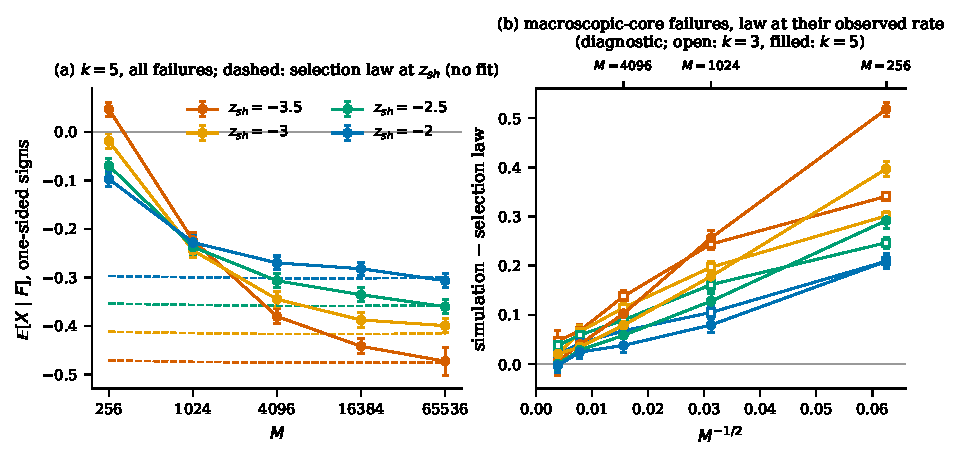
\includegraphics[width=\linewidth]{figures/fig_convergence.pdf}
\caption{Conditional mean and convergence diagnostics. Left: all failures for $k=5$, with analytic selection predictions at $z_{\rm sh}$. Right: macro-core conditional means minus predictions at their observed failure rates. The empirical coordinate in the right panel makes it a diagnostic rather than a parameter-free test of the marginal failure law.}
\label{fig:convergence}
\end{figure}

\subsection{Central-window calibration}
Figure~\ref{fig:calib} compares nominal and actual lower-tail probabilities. In the tested one-sided central-window configurations with failure probability at least about $0.03$, the additive selection/chi-square rule reduces grouped RMS relative error to roughly $0.04$--$0.08$ for $M\ge256$. Unconditional thresholds retain substantial selection error.

These are grouped empirical summaries, not bounds on individual configurations. Group composition varies with $M$. The theorem explains the persistent selection effect and its direction, while the finite-size comparison evaluates a particular approximation on the tested configurations.
\begin{figure}[!htbp]
\centering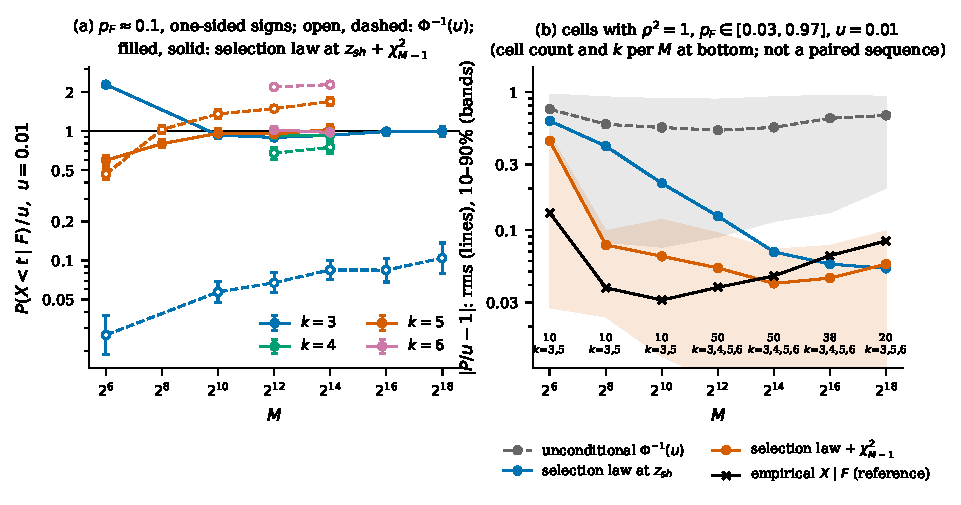
\includegraphics[width=\linewidth]{figures/fig_calib.pdf}
\caption{Central-window lower-tail calibration. Panel (a) shows representative configurations near failure probability $0.1$; panel (b) aggregates one-sided configurations with failure probabilities between $0.03$ and $0.97$. Dispersion and configuration counts accompany the grouped RMS values. Empirical thresholds use training trials; full-record risks use disjoint failed test trials.}
\label{fig:calib}
\end{figure}

\subsection{Deep-left-tail limitations}
Figure~\ref{fig:leftrisk} illustrates the boundary of finite-size accuracy. At $k=5$, $M=65536$, and $z_{\rm sh}\approx-3.5$, the corrected nominal $1\%$ threshold gives 52 lower-tail observations among 4549 failures: $1.14\%$, with a $95\%$ Wilson interval of $[0.87\%,1.50\%]$. The corresponding $k=3$ configuration gives 273 of 9021, or $3.03\%$, with interval $[2.69\%,3.40\%]$. Restricting the latter to macro-core failures gives approximately $0.71\%$.

Small-core failures remain consequential at these finite sizes. Macro-core dominance alone is not sufficient either: the $k=5$, $M=256$ deep-left-tail point is almost entirely macro-core failure, yet its corrected $1\%$ threshold gives only about $0.31\%$. Both conditional-distribution error and small-core contamination matter. No error-floor theorem is asserted.
\begin{figure}[!htbp]
\centering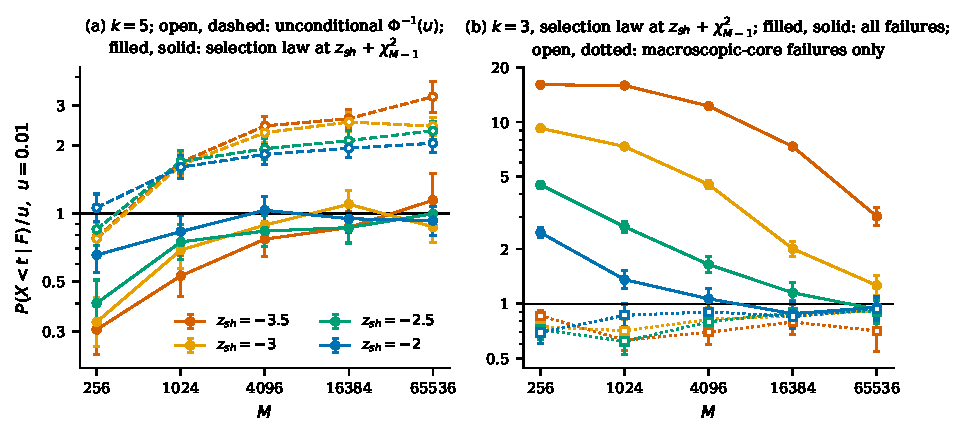
\includegraphics[width=\linewidth]{figures/fig_leftrisk.pdf}
\caption{Actual lower-tail probabilities in the deep-left-tail series, divided by the nominal level $u=0.01$. All-failure and macro-core layers are distinguished in panel (b). These analytic thresholds use no empirical training quantile; intervals reflect binomial uncertainty in the observed failures.}
\label{fig:leftrisk}
\end{figure}

\section{Discussion}
Failure-conditioned measurement exhibits a selection effect that survives standardization for unbalanced signs. Its strength is determined by the explicit correlation $\eta_k\rho^2$, and its direction changes between $k=4$ and $k=5$. Improving the unconditional reference distribution alone therefore cannot remove the failure-selection effect.

The theoretical regime fixes $k\ge3$ and considers ideal Plain mappings, deterministic signs independent of the mapping, and a nondegenerate critical-window limit. Balanced-selection invariance applies more broadly at positive density. Finite-size error rates, rare-failure windows, growing $k$, nonideal checksums, and adaptive procedures with unknown load remain open.

A standardized chi-square reference becomes asymptotically normal as $M$ grows. This is compatible with the normal marginal limit but does not establish an exact chi-square law at finite critical loads. Accordingly, the additive rule~\eqref{eq:selchi} remains a numerical approximation.

The interactive laboratory visualizes the degree-one trajectory, its local bottleneck scaling, a drift-corrected backward functional, and accumulated fluctuations for Plain and configuration mappings. Its one-step compensation uses a first-order partner law; the plotted residual is an approximation to the Doob martingale. Standard deviations are shown only while at least $99\%$ of sampled paths remain active, which limits but does not eliminate survivor selection. These visualizations explain the mechanism and complement, rather than replace, the limit arguments and larger numerical experiments.

\appendix
\section{A finite-composition variance check}
For a fixed weighted overlap graph on $n=d\ge4$ vertices, let $A=\sum_i l_i^2$ and define
\begin{align}
a_2&=\frac{n^2\rho_M^2-n}{n(n-1)},\\
a_4&=\frac{(n\rho_M)^4-(6n-8)(n\rho_M)^2+3n(n-2)}
{n(n-1)(n-2)(n-3)}.
\end{align}
These are the products of two and four distinct fixed-composition signs, averaged over uniform assignments. Expanding pairs of overlap edges by whether they coincide, share one vertex, or are disjoint gives
\begin{align}
\E_s[Y_s\mid\mathcal G_M]&=a_2W,\\
\Var_s(Y_s\mid\mathcal G_M)
&=B(1-2a_2+a_4)+A(a_2-a_4)+W^2(a_4-a_2^2).
\end{align}
The expansions
$a_2=\rho_M^2-(1-\rho_M^2)/n+O(n^{-2})$ and
$a_4=\rho_M^4-6\rho_M^2(1-\rho_M^2)/n+O(n^{-2})$
recover the limiting variance in the fixed-sign argument. This identity checks the total-composition correction independently of the CLT.

\begin{thebibliography}{9}
\bibitem{dm} A. Dembo and A. Montanari, ``Finite size scaling for the core of large random hypergraphs,'' \emph{The Annals of Applied Probability}, 2008.
\bibitem{amru} A. Amraoui, A. Montanari, T. Richardson, and R. Urbanke, ``Finite-Length Scaling for Iteratively Decoded LDPC Ensembles,'' \emph{IEEE Transactions on Information Theory}, 2009.
\bibitem{nks} T. Nozaki, K. Kasai, and K. Sakaniwa, ``Analytical Solution of Covariance Evolution for Irregular LDPC Codes,'' 2012.
\bibitem{jl} S. Janson and M. {\L}uczak, ``Asymptotic normality of the k-core in random graphs,'' \emph{The Annals of Applied Probability}, 2008.
\end{thebibliography}
\end{document}
